\documentclass[tikz,border=5mm]{standalone}
\usepackage{tikz}
\usetikzlibrary{calc}
\begin{document}
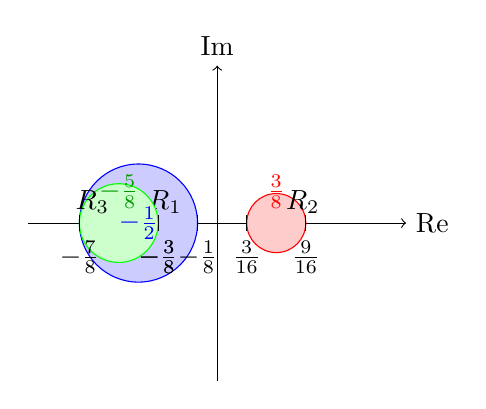
\begin{tikzpicture}[scale=2]
  % Define the centers and radii of the circles
  \def\centerROne{-0.5}
  \def\radiusROne{0.375}
  \def\centerRTwo{0.375}
  \def\radiusRTwo{0.1875}
  \def\centerRThree{-0.625}
  \def\radiusRThree{0.25}
  
  % Draw the axes
  \draw[->] (-1.2,0) -- (1.2,0) node[right] {Re};
  \draw[->] (0,-1) -- (0,1) node[above] {Im};

  % Draw the circles
  \draw[blue,fill=blue!20] (\centerROne,0) circle (\radiusROne) node[above right, black] {$R_1$};
  \draw[red,fill=red!20] (\centerRTwo,0) circle (\radiusRTwo) node[above right,black] {$R_2$};
  \draw[green,fill=green!20] (\centerRThree,0) circle (\radiusRThree) node[above left, black] {$R_3$};

  % Mark the boundaries of the intervals on the real axis
  \foreach \x/\xtext in {-0.875/-\frac{7}{8}, -0.125/-\frac{1}{8}, 0.1875/\frac{3}{16}, 0.5625/\frac{9}{16}, -0.375/-\frac{3}{8}, -0.375/-\frac{3}{8}}
  {
    \draw (\x,0.05) -- (\x,-0.05) node[below] {$\xtext$};
  }

  % Add some labels for the centers
  \node[blue] at (\centerROne,0) {$-\frac{1}{2}$};
  \node[red] at (\centerRTwo,0.2) {$\frac{3}{8}$};
  \node[green!60!black] at (\centerRThree,0.2) {$-\frac{5}{8}$};
\end{tikzpicture}
\end{document}